\documentclass[DaoFP]{subfiles}
\begin{document}
\setcounter{chapter}{10}

\chapter{Dependent Types}

We've seen types that depend on other types. They are defined using type constructors with type parameters, like \hask{Maybe} or \hask{[]}. Most programming languages have some support for generic data types---data types parameterized by other data types.

Categorically, such types are modeled as functors \footnote{A type constructor that has no \hask{Functor} instance can be thought of as a functor from a discrete category---a category with no arrows other than identities}.

A natural generalization of this idea is to have types that are parameterized by values. For instance, it's often advantageous to encode the length of a list in its type. A list of length zero would have a different type than a list of length one, and so on. 

Types parameterized by values are called \emph{dependent types}. There are languages like Idris or Agda that have full support for dependent types. It's also possible to implement dependent types in Haskell, but support for them is still rather patchy.

\section{Dependent Vectors}

We'll start with the standard example of a counted list, or a vector:
\begin{haskell}
data Vec n a where
    VNil  :: Vec Z a
    VCons :: a -> Vec n a -> Vec (S n) a
\end{haskell}
The compiler will recognize this definition as dependently typed if you include the following language pragmas:
\begin{haskell}
{-# LANGUAGE DataKinds #-}
{-# LANGUAGE GADTs #-}
\end{haskell}
The first argument to the type constructor is a natural number \hask{n}. Notice: this is a value, not a type. The type checker figures that out from the usage in the two data constructors. The first one creates a vector of the type \hask{Vec Z a}, and the second creates a vector of the type \hask{Vect (S n) a}, where \hask{Z} and \hask{S} are defined as the constructors of natural numbers:
\begin{haskell}
data Nat = Z | S Nat
\end{haskell}

We can be more explicit about the parameters if we use the pragma:
\begin{haskell}
{-# LANGUAGE KindSignatures #-}
\end{haskell}
and import the library:
\begin{haskell}
import Data.Kind
\end{haskell}
We can then specify that \hask{n} is a \hask{Nat}, whereas \hask{a} is a \hask{Type}:
\begin{haskell}
data Vec (n :: Nat) (a :: Type) where
    VNil  :: Vec Z a
    VCons :: a -> Vec n a -> Vec (S n) a
\end{haskell}

Using one of these definitions we can, for instance, construct a vector (of integers) of length zero:
\begin{haskell}
emptyV :: Vec Z Int
emptyV = VNil
\end{haskell}
It has a different type than a vector of length one:
\begin{haskell}
singleV :: Vec (S Z) Int
singleV = VCons 42 VNil
\end{haskell}
and so on.

We can now define a dependently typed function that returns the first element of a vector:
\begin{haskell}
headV :: Vec (S n) a -> a
headV (VCons a _) = a
\end{haskell}
This function is guaranteed to work exclusively with non-zero-length vectors. These are the vectors whose size matches \hask{(S n)}, which cannot be \hask{Z}. If you try to call this function with \hask{emptyV}, the compiler will flag the error.

Another example is a function that zips two vectors together. Encoded in its type signature is the requirement that the two vectors be of the same size \hask{n} (the result is also of the size \hask{n}):
\begin{haskell}
zipV :: Vec n a -> Vec n b -> Vec n (a, b)
zipV (VCons a as) (VCons b bs) = VCons (a, b) (zipV as bs)
zipV VNil VNil = VNil
\end{haskell}

\begin{exercise}
Implement the function \hask{tailV} that returns the tail of the non-zero-length vector. Try calling it with \hask{emptyV}.
\end{exercise}

\section{Dependent Types Categorically}

The easiest way to visualize dependent types is to think of them as families of types indexed by elements of a set. In the case of counted vectors, the indexing set would be the set of natural numbers.

The zeroth type would be the unit type \hask{()} representing an empty vector. The type corresponding to one would be \hask{a}; then we'd have a pair \hask{(a, a)}, a triple \hask{(a, a, a)} and so on, with higher and higher powers of \hask{a}.

If we want to talk about the whole family as one big set, we can take the union of all these types.

\subsection{Fibrations}

Although intuitively easy to visualize, this point of view doesn't generalize nicely to category theory, where we don't like mixing sets with objects. So we turn this picture on its head and instead of talking about injecting family members into the family, we consider a mapping that goes in the opposite direction. 

This, again, we can first visualize using sets. We have one big set $E$ describing the whole family and a function $p$ called the projection that goes from $E$ down to the indexing set $B$ (also called the \emph{base}). 

This function will, in general, map multiple elements to one. We can then talk about the inverse image of a particular element $x \in B$ as the set of elements that get mapped down to it by $p$. This set is called the \emph{fibre} and is written $p^{-1} x$ (even though, in general, $p$ is not invertible in the normal sense).

\[
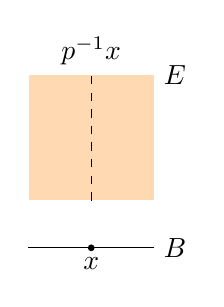
\begin{tikzpicture}

\def\yb{0}; % base
\def\yfb{0.6}; % fiber bottom
\def\yft{2.2}; % fiber top

\def\dx{0.8};

\def\xbl{0};
\def\xbm{\xbl + \dx};
\def\xbr{\xbl + 2*\dx};

\filldraw[fill=orange!30, draw=white] (\xbl, \yfb) rectangle (\xbr, \yft);

\draw (\xbl, \yb) -- (\xbr, \yb);

\draw[dashed] (\xbm, \yfb) -- (\xbm, \yft);

\filldraw[black] (\xbm, \yb) circle (1 pt);
\node[below] at (\xbm, \yb) {$x$};
\node[above] at (\xbm, \yft) {$p^{-1} x$};
\node[right] at (\xbr, \yb) {$B$};
\node[right] at (\xbr, \yft) {$E$};

\end{tikzpicture}
\]


Now forget about sets. A \emph{fibration} in an arbitrary category is a pair of objects $E$ and $B$ and an arrow $p \colon E \to B$. 

So this is really just an arrow, but the context is everything. When an arrow is called a fibration, use the intuition from sets, and imagine its source $E$ as a collection of fibers, with $p$ projecting each fiber down to a single point in the base $B$. 

We will model type families as fibrations. For instance, our counted-vector family can be represented as a fibration whose base is the type of natural numbers. The whole family is a sum (coproduct) of consecutive powers (products) of $A$:
\[ E = \coprod_{n\colon \mathbb{N}} A^n \]
the zeroth power---the initial object---representing a vector of size zero.
\[
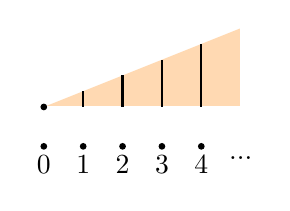
\begin{tikzpicture}
\def\dx{0.5};
\def\yb{0};
\def\dy{0.2};
\def\y{0.5};

\filldraw[fill=orange!30, draw=white] (0, \y) to (5* \dx, \y) to (5*\dx, \y + 5*\dy);

\filldraw[black] (0, 0) circle (1 pt);
\node[below] at (0, 0) {$0$};
\filldraw[black] (0, \y) circle (1 pt);

\filldraw[black] (\dx, 0) circle (1 pt);
\node[below] at (\dx, 0) {$1$};
\draw[thick] (\dx, \y) -- (\dx, \y + \dy);

\filldraw[black] (2*\dx, 0) circle (1 pt);
\node[below] at (2*\dx, 0) {$2$};
\draw[thick] (2*\dx, \y) -- (2*\dx, \y + 2* \dy);

\filldraw[black] (3*\dx, 0) circle (1 pt);
\node[below] at (3*\dx, 0) {$3$};
\draw[thick] (3*\dx, \y) -- (3*\dx, \y + 3* \dy);

\filldraw[black] (4*\dx, 0) circle (1 pt);
\node[below] at (4*\dx, 0) {$4$};
\draw[thick] (4*\dx, \y) -- (4*\dx, \y + 4* \dy);
\node[below] at (5*\dx, 0) {$...$};

\end{tikzpicture}
\]

The projection $p$ is a mapping out of a sum, so it can be defined as a product of individual mappings $A^n \to \mathbb{N}$, each assigning the number corresponding to the power to which $A$ was raised.

\subsection{Slice categories}

In category theory we like to describe things in bulk---defining internal structure of things by structure-preserving mappings between them. Such is the case with fibrations. 

If we fix the base object $B$ and consider all possible source objects in $\mathcal{C}$, and all possible projections down to $B$, we get a \emph{slice category} $\mathcal{C}/B$ (also known as an over-category). 

An arrow in the slice category between two objects $\langle E, p \rangle$ and $\langle E', p' \rangle$ is an arrow $f \colon E \to E'$ that commutes with the projections, that is:
\[p' \circ f = p \]

Again, the best way to visualize this is to notice that such an arrow maps fibers of $p$ to fibers of $p'$. It's a ``fiber-preserving'' mapping.

\[
 \begin{tikzcd}
 E
 \arrow[rd, "p"']
 \arrow[rr, "f"]
 && E'
 \arrow[ld, "p'"]
 \\
 &B
  \end{tikzcd}
\]


\subsection{Pullbacks}

 Let's start with a particular fibration $p \colon E \to B$ and ask ourselves the question: what happens when we change the base from $B$ to some $B'$ that is related to it through a mapping $f \colon B' \to B$. Can we ``pull the fibres back'' along $f$? 
 
 Again, let's think about sets first. Imagine picking a fibre in $E$ over some point $y \in B$. We can plant this fibre over all points in $B'$ that are in the inverse image $f^{-1} y$. If multiple points in $B'$ are mapped to the same point in $B$, we just duplicate the corresponding fiber. This way every point in $B'$ will have a fiber sticking out of it. The union of all these fibers will form a new set $E'$.

\[
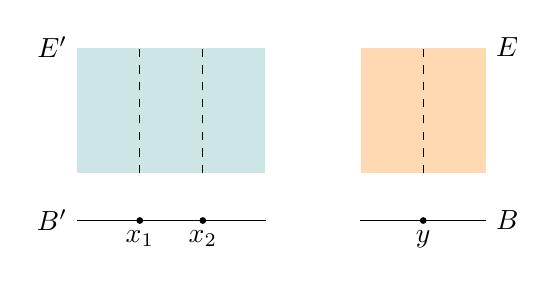
\begin{tikzpicture}

\def\yb{0}; % base
\def\yfb{0.6}; % fiber bottom
\def\yft{2.2}; % fiber top

\def\dx{0.8};

\def\xal{-1.8};
\def\xam{\xal + \dx};
\def\xamm{\xal + 2 * \dx};
\def\xar{\xal + 3*\dx};

\def\xbl{1.8};
\def\xbm{\xbl + \dx};
\def\xbr{\xbl + 2*\dx};

\filldraw[fill=blue!50!green!20, draw=white] (\xal, \yfb) rectangle (\xar, \yft);
\filldraw[fill=orange!30, draw=white] (\xbl, \yfb) rectangle (\xbr, \yft);

\draw (\xal, \yb) -- (\xar, \yb);
\draw (\xbl, \yb) -- (\xbr, \yb);

\draw[dashed] (\xam, \yfb) -- (\xam, \yft);
\draw[dashed] (\xamm, \yfb) -- (\xamm, \yft);
\draw[dashed] (\xbm, \yfb) -- (\xbm, \yft);

\filldraw[black] (\xam, \yb) circle (1 pt);
\filldraw[black] (\xamm, \yb) circle (1 pt);
\filldraw[black] (\xbm, \yb) circle (1 pt);
\node[below] at (\xbm, \yb) {$y$};
\node[right] at (\xbr, \yb) {$B$};
\node[left] at (\xal, \yb) {$B'$};
\node[right] at (\xbr, \yft) {$E$};
\node[left] at (\xal, \yft) {$E'$};
\node[below] at (\xam, \yb) {$x_1$};
\node[below] at (\xamm, \yb) {$x_2$};

\end{tikzpicture}
\]

We have constructed a new fibration with the base $B'$. Its projection $p' \colon E' \to B'$ maps each point in a fibre to the point over which this fibre was planted. There is also a natural mapping $g \colon E' \to E$ that maps fibers to their corresponding fibres. 

By construction, this new fibration $\langle E', p'\rangle$ satisfies the condition:
\[ p \circ g = f \circ p' \]
which can be represented as a commuting square:
\[
 \begin{tikzcd}
 E'
 \arrow[d, "p'"']
 \arrow[r, "g"]
 & E
 \arrow[d, "p"]
 \\
 B'
 \arrow[r, "f"]
 &B
  \end{tikzcd}
\]

In  $\mathbf{Set}$, we can explicitly construct $E'$ as a subset of the cartesian product $B' \times E$ with $p' = \pi_1$ and $g = \pi_2$ (the two cartesian projections). An element of $E'$ is a pair $\langle b, e \rangle$, and the commuting condition is the equation:
\[ f b = p e \]

This commuting square is the starting point for the categorical generalization. However, even in $\mathbf{Set}$ there are many different fibrations over $B'$ that make this diagram commute. We have to pick the universal one. Such a universal construction is called a \emph{pullback}, or a \emph{fibered product}.

A pullback of $p \colon E \to B$ along $f \colon B' \to B$ is an object $E'$ together with two arrows $p' \colon E' \to B'$ and $g \colon E' \to E$ that makes the above diagram commute and that satisfies the universal condition. 

The universal condition says that, for any other candidate object $G$ with two arrows $q \colon G \to E$ and $q' \colon G \to B'$ making the square commute, there is a unique arrow $h \colon G \to E'$ that makes the whole diagram commute:

\[
 \begin{tikzcd}
 G
 \arrow[dr, dashed, "h"]
 \arrow[drr, bend left, "q"]
 \arrow[ddr, bend right, "q'"']
 \\
 &E'
 \arrow[r, "g"]
 \arrow[d, "p'"']
\arrow[dr, phantom,  , very near start, "\lrcorner"]
 &E
 \arrow[d, "p"]
 \\
 &B'
 \arrow[r, "f"]
 &B
  \end{tikzcd}
\]
The little corner symbol is often used to mark pullbacks.

It's worth noting that picking the terminal object as the pullback target gives us the definition of the categorical product:
\[
 \begin{tikzcd}
 B \times E
 \arrow[d, "\pi_1"']
 \arrow[r, "\pi_2"]
\arrow[dr, phantom,  , very near start, "\lrcorner"]
 & E
 \arrow[d, "!"]
 \\
 B
 \arrow[r, "!"]
 &
 1
  \end{tikzcd}
\]

Conversely, a single fiber can be extracted from a fibration by pulling it back to the terminal object. In this case the mapping $x \colon 1 \to B$ picks an element of the base, and the pullback along it pulls a fiber $F$:
\[
 \begin{tikzcd}
 F
 \arrow[d, "!"']
 \arrow[r, "g"]
\arrow[dr, phantom,  , very near start, "\lrcorner"]
 & E
 \arrow[d, "p"]
 \\
 1
 \arrow[r, "x"]
 &
 B
  \end{tikzcd}
\]
The arrow $g$ injects this fibre back into $E$. By varying $x$ we can pick different fibers in $E$.

\begin{exercise}
Show that a pullback can be defined as a limit of the diagram from a stick-figure category with three objects:
\[ A \rightarrow B \leftarrow C \]
\end{exercise}

\subsection{Base-change functor}

We used a cartesian closed category as a model for programming. To model dependent types, we need to impose an additional condition: We require the category to be \emph{locally cartesian closed}. This is a category in which all slice categories are cartesian closed. 

In particular, such categories have all pullbacks, so it's always possible to change the base of any fibration.  Base change induces a mapping between slice categories that is functorial. 

Given two slice categories $\mathcal{C}/B'$ and $\mathcal{C}/B$ and an arrow between bases $f \colon B' \to B$ the base-change functor $f^* \colon \mathcal{C}/B \to \mathcal{C}/B'$ maps a fibration $\langle E, p \rangle$ to the fibration $\langle E', f^* p' \rangle$, which is given by the pullback:
\[
 \begin{tikzcd}
 E'
\arrow[dr, phantom,  , very near start, "\lrcorner"]
 \arrow[d, "f^*p"']
 \arrow[r, "g"]
 & E
 \arrow[d, "p"]
 \\
 B'
 \arrow[r, "f"]
 &B
  \end{tikzcd}
\]
Notice that the functor $f^*$ goes in the opposite direction to the arrow $f$.

In a locally cartesian closed category, the base change functor has both the left and the right adjoints. The left adjoint is called the dependent sum, and the right adjoint is called the dependent product.


\section{Dependent Sum}

In type theory, the dependent sum or the sigma type is defined as a pair of values in which the type of the second component depends on the value of the first component. Our counted vector can be thought of as a dependent sum consisting of a natural number \hask{n} paired with an n-tuple of \hask{a}.

The introduction rule for the dependent sum assumes that there is a family of types $T(x)$ indexed by elements of some base type $B$. Then an element of $\Sigma_{x : B} T(x)$ is constructed from a pair of elements $x \colon B$ and $y \colon T(x)$. 

Categorically, dependent sum is modeled as the left adjoint of the base-change functor. To see this, let's first revisit the definition of a product. We've seen before that it can be written as a pullback from the terminal object. Here's the universal construction for the product/pullback (the weird notation anticipates the ultimate goal of this construction):
\[
 \begin{tikzcd}
 G
 \arrow[dr, dashed, "\phi^T"]
 \arrow[drr, bend left, "\phi"]
 \arrow[ddr, bend right, "q"]
 \\
 &B' \times E
\arrow[dr, phantom,  , very near start, "\lrcorner"]
 \arrow[r, "\pi_2"]
 \arrow[d, "\pi_1"']
 &E
 \arrow[d, "!"]
 \\
 &B'
 \arrow[r, "!"]
 &1
  \end{tikzcd}
\]

We have also seen the product defined using an adjunction. We can spot the adjunction in this diagram: for every pair of arrows $\langle \phi, q \rangle$ there is a unique arrow $\phi^T$ that makes the triangles commute. 

Notice that, if we keep $q$ fixed, we get a one-to-one correspondence between two arrows $\phi$ and $\phi^T$. 

We can now put on our fibrational glasses on and notice that $\langle G, q\rangle$ and $\langle B' \times E, \pi_1 \rangle$ are two fibrations over the same base $B'$, and the commuting triangle makes $\phi^T$ a morphism in the slice category $\mathcal{C}/B'$. In other words $\phi^T$ is a member of the hom-set:
 \[ (\mathcal{C}/B')(\langle G, q \rangle, \langle B' \times E, \pi_1 \rangle)  \]
 
 We can now rewrite the one-to-one correspondence between $\phi$ and $\phi^T$ as an isomorphism of hom-sets:
\[ \mathcal{C}(G, E) \cong  (\mathcal{C}/B')(\langle G, q \rangle, \langle B' \times E, \pi_1 \rangle)\]
In fact, it's an adjunction in which the left functor is the forgetful functor that maps $\langle G, q \rangle$ to $G$.

We can now generalize this diagram by replacing the terminal object with an arbitrary base $B$. We now have a fibration $\langle E, p \rangle$, and we get the pullback square that defines the base-change functor:
\[
 \begin{tikzcd}
 G
 \arrow[dr, dashed, "\phi^T"]
 \arrow[drr, bend left, "\phi"]
 \arrow[ddr, bend right, "q"]
 \\
 &E'
\arrow[dr, phantom,  , very near start, "\lrcorner"]
 \arrow[r, "g"]
 \arrow[d, "f^* p"']
 &E
 \arrow[d, "p"]
 \\
 &B'
 \arrow[r, "f"]
 &B
  \end{tikzcd}
\]

\[ (\mathcal{C}/B) \big(\langle G, \Sigma_f q\rangle , \langle E, p\rangle \big)  \cong   (\mathcal{C}/B') (\langle G, q \rangle , \langle E', f^* p\rangle )\]
\[
\begin{tikzcd}
 G
 \arrow[rr, "\phi^T"]
 \arrow[rd, "q"']
 && E'
 \arrow[ld, "f^* p"]
 \\
 & B'
  \end{tikzcd}
 \hspace{20pt}
 \begin{tikzcd}
 G
 \arrow[rr, "\phi"]
 \arrow[rd, "\Sigma_f q"']
 &&E
 \arrow[dl, "p"]
 \\
 &B
  \end{tikzcd}
\]

\[ \Sigma_f q = f \circ q \]


\[
 \begin{tikzcd}
 1
 \arrow[dr, dashed, "y"]
 \arrow[drr, bend left, "\phi"]
 \arrow[ddr, bend right, "id"']
 \\
 &F
 \arrow[r, "g"]
 \arrow[d, "!"']
 &E
 \arrow[d, "p"]
 \\
 &1
 \arrow[r, "x"]
 &B
  \end{tikzcd}
\]


left adjoint to base-change functor

proof by universal property of pullbacks

terminal-object base picks a fiber

terminal-object as bundle over termina-object base: picks en element of a given fiber


\section{Dependent Product}

\[
 \begin{tikzcd}
 G \times B
 \arrow[d, "\phi^T \times B"']
 \arrow[dr, "\phi"]
 \\
 S \times B
 \arrow[r, "\varepsilon"]
 &E
  \end{tikzcd}
\]


Bundle $E/B$ (can be thought of as a sum of fibres).

Family of sections $S$ of a bundle $E$ over $B$. Equipped with a projection $p \colon E \to B$.

Evaluation map $\varepsilon \colon S \times B \to E$ must commute with projection, so it's an arrow in $\mathbf{Set}/B$.

Universal property: For any other set $G$ and a mapping in $\mathbf{Set}/B$,  $\phi \colon G \times B \to E$, there is a unique mapping $\phi^T \colon G \to S$ that makes things commute.

\[\mathbf{Set} (G, S) \cong (\mathbf{Set}/B)(\langle G\times B, \pi_2\rangle , \langle E, p\rangle ) \]
\[\pi_2 \colon G \times B \to B \]
\[p \colon E \to B \]

this can be written as:

\[(\mathbf{Set}/1) (\langle G, !\rangle , \langle S, !\rangle ) \cong (\mathbf{Set}/B)(\langle G\times B, \pi_2\rangle , \langle E, p\rangle )  \]

$G \times B$ is a pullback from the terminal object
\[
 \begin{tikzcd}
 G \times B
 \arrow[d, "\pi_2"]
 \arrow[r, "\pi_1"]
 & G
 \arrow[d, "!"]
 \\
 B
 \arrow[r, "!"]
 &
 1
  \end{tikzcd}
\]

Given $f \colon B \to B'$, we have the base-changer functor $f^* \colon \mathcal{C}/B' \to \mathcal{C}/B$.

$\Pi_f \colon \mathcal{C}/B \to \mathcal{C}/B'$ is right adjoint to $f^*$

\[(\mathcal{C}/B')(\langle G, q \rangle, \langle S, \Pi_f \,p\rangle) \cong (\mathcal{C}/B) (\langle G', f^* q\rangle, \langle E, p \rangle) \]

\[
\begin{tikzcd}
 G
 \arrow[rr, "\phi^T"]
 \arrow[rd, "q"']
 && S
 \arrow[ld, "\Pi_f \, p"]
 \\
 & B'
  \end{tikzcd}
 \hspace{20pt}
 \begin{tikzcd}
 G'
 \arrow[rr, "\phi"]
 \arrow[rd, "f^* q"']
 &&E
 \arrow[dl, "p"]
 \\
 &B
  \end{tikzcd}
\]

\[
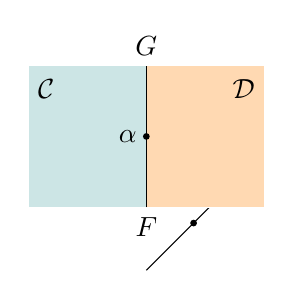
\begin{tikzpicture}
\def\dy{0.6};
\def\ybl{0}; % base left
\def\ybm{\dy}; % base middle
\def\ybr{2*\dy}; % base right

\def\dx{0.6};
\def\xbl{0};
\def\xbm{\dx};
\def\xbr{2*\dx};

\draw (\xbl, \ybl) -- (\xbr, \ybr);
\filldraw[black] (\xbm, \ybm) circle (1 pt);



\def\x{0};
\def\xl{-1.5};
\def\xr{1.5};


\def \ya{0.8};
\def \yb{1.7};
\def \yc{2.6};
\def \yt {2.3};

\filldraw[fill=blue!50!green!20, draw=white] (\xl, \ya) rectangle (\x, \yc);
\filldraw[fill=orange!30, draw=white] (\x, \ya) rectangle (\xr, \yc);

\node[below] (a) at (\x, \ya) {$F$};
\node(b) at (\x, \yb) {};
\node [above] (c) at (\x, \yc) {$G$};

\node(l)[right] at (\xl, \yt) {$\mathcal{C}$};
\node(r)[left] at (\xr, \yt) {$\mathcal{D}$};


\filldraw[black] (b) circle (1 pt);
\node [left] at (b) {$\alpha$};

\draw (a)  -- (c);

\end{tikzpicture}
\]

\section{Equality}

Our first experience in mathematics is related to equality. We learn that 
\[1+1=2\] 
and we don't think much of it afterwards. 

But what does it mean that $1+1$ is equal to $2$? Two is a number, but one plus one is an expression, so they are not the same thing. There is some mental processing that we have to perform before we pronounce these two things equal. 

Contrast this with the statement $0 = 0$, in which both sides of equality are \emph{the same thing}. If we are to define equality, we'll have to at least make sure that every thing is equal to itself. We call this property \emph{reflexivity}. 

Recall our definition of natural numbers:
\begin{haskell}
data Nat where
  Z :: Nat
  S :: Nat -> Nat
\end{haskell}
This is the definition of equality for natural numbers:
\begin{haskell}
equal :: Nat -> Nat -> Bool
equal Z Z = True
equal (S m) (S n) = equal m n
equal _ _ = False
\end{haskell}
We are recursively stripping $S$'s in each number until one of them reaches $Z$. If the other reaches $Z$ at the same time, the numbers were equal, otherwise they were not. 

\subsection{Equational reasoning}

Notice that when defining equality we were already using the equal sign. For instance, the equal sign in:
\begin{haskell}
equal Z Z = True
\end{haskell}
tells us that wherever we see the expression \hask{equal Z Z} we can replace it with \hask{True} and vice versa. This is the principle of substituting equals for equals, which is the basis for \emph{equational reasoning} in Haskell. We can't encode proofs of equality directly in Haskell, but we can use equational reasoning to reason about Haskell programs. This is one of the main advantages of pure functional programming. You can't perform such substitutions in imperative languages, because of side effects.

If we want to prove that $1+1$ is $2$, we have to first define addition. The definition can either be recursive in the first or in the second argument. This one recurses in the second argument:
\begin{haskell}
add :: Nat -> Nat -> Nat
add n Z = n
add n (S m) = S (add n m)
\end{haskell}
We encode $1 + 1$ as 
\begin{haskell}
add (S Z) (S Z)
\end{haskell}
We can now use the definition of \hask{add} to simplify this expression. We try to match the first clause and fail, because \hask{S Z} is not the same as \hask{Z}. But the second clause matches. We get:
\begin{haskell}
add (S Z) (S Z) = S (add (S Z) Z)
\end{haskell}
In this expression we can perform another substitution of equals:
\begin{haskell}
add (S Z) Z = S Z
\end{haskell}
to arrive at:
\begin{haskell}
add (S Z) (S Z) = S (S Z)
\end{haskell}
We can clearly see that this is the same as our encoding of $2$. But we haven't shown that our definition of equality is reflexive so, in principle, we don't know of \hask{eq (S (S Z)) (S (S Z))} yields \hask{True}. We have to use step-by-step equational reasoning again:
\begin{haskell}
equal (S (S Z) (S (S Z)) =
{- second clause of the definition of equal -}
equal (S Z) (S Z) =
{- second clause of the definition of equal -}
equal Z Z =
{- first clause of the definition of equal -}
True
\end{haskell}

We can use this kind of reasoning to prove statements about concrete numbers, but we run into problems when reasoning about arbitrary numbers. For instance, using our definition of addition, we can easily show that \hask{add n Z} is the same as \hask{n}. But we can't prove that \hask{add Z n} is the same as \hask{n}. Such proofs require the use of induction. 

We end up distinguishing between two kinds of equality. One is proven using substitutions, or rewriting rules, and is called \emph{definitional equality}. You can think of it as macro expansion or inline expansion in programming languages. It also involves $\beta$-reductions: performing function application by replacing formal parameters by actual arguments, as in:
\begin{haskell}
(\x -> x + x) 2 =
{- beta reduction -}
2 + 2
\end{haskell}

The second more interesting kind of equality is called \emph{propositional equality} and it may require actual proofs. 

\subsection{Equality vs isomorphism}

We talked about category theorists preferring isomorphism over equality---at least as it comes to objects. It is true that, within the confines of a category, there is no way to differentiate between isomorphic objects. In general, though, equality is stronger than isomorphism. This is a problem, because it's very convenient to be able to substitute equals for equals, but it's not always clear that one can substitute isomorphic for isomorphic. 

Mathematicians have been struggling with this problem, trying to modify the definition of isomorphism, but a real breakthrough came when they decided to simultaneously weaken the definition of equality. This led to the development of \emph{homotopy type theory}, or HoTT for short. 

Roughly speaking, in HoTT, equality is represented as a type, and in order to prove equality one has to construct an element of that type---in the spirit of the Curry-Howard interpretation. Furthermore, the proofs themselves can be compared for equality, and so on ad infinitum. You can picture this by considering proofs of equality not as points but as some abstract paths that can be morphed into each other; hence the language of homotopies.

In this setting, instead of isomorphism, which involves strict equalities of arrows:
\[ f \circ g = id \]
\[ g \circ f = id \]
one defines an equivalence, in which these equalities are treated as equality types.

The main idea of HoTT is that one can impose the \emph{univalence axiom}, which states that equalities are equivalent to equivalences, or symbolically:
\[ (A = B) \cong (A \cong B) \]

\subsection{Equality types}

\subsection{Notes}


relation to logic: universal/esistential quantification


induction

\begin{exercise}
\end{exercise}

\begin{haskell}
\end{haskell}

\[
 \begin{tikzcd}
  \end{tikzcd}
\]

\[   \mathbf{Set} \]
\[   \mathcal{C} \]

\end{document}